\let\negmedspace\undefined
\let\negthickspace\undefined
\documentclass[journal]{IEEEtran}
\usepackage[a5paper, margin=10mm, onecolumn]{geometry}
\usepackage{lmodern} % Ensure lmodern is loaded for pdflatex
\usepackage{tfrupee} % Include tfrupee package

\setlength{\headheight}{1cm} % Set the height of the header box
\setlength{\headsep}{0mm}     % Set the distance between the header box and the top of the text

\usepackage{gvv-book}
\usepackage{gvv}
\usepackage{cite}
\usepackage{amsmath,amssymb,amsfonts,amsthm}
\usepackage{algorithmic}
\usepackage{graphicx}
\usepackage{textcomp}
\usepackage{xcolor}
\usepackage{txfonts}
\usepackage{listings}
\usepackage{enumitem}
\usepackage{mathtools}
\usepackage{gensymb}
\usepackage{comment}
\usepackage[breaklinks=true]{hyperref}
\usepackage{tkz-euclide} 
\usepackage{listings}
% \usepackage{gvv}                                        
\def\inputGnumericTable{}                                 
\usepackage[latin1]{inputenc}                                
\usepackage{color}                                            
\usepackage{array}                                            
\usepackage{longtable}                                       
\usepackage{calc}                                             
\usepackage{multirow}                                         
\usepackage{hhline}                                           
\usepackage{ifthen}                                           
\usepackage{lscape}
\begin{document}

\bibliographystyle{IEEEtran}
\vspace{3cm}

\title{4.4.33}
\author{EE24BTECH11019 - DWARAK A}
% \maketitle
% \newpage
% \bigskip
{\let\newpage\relax\maketitle}

\renewcommand{\thefigure}{\theenumi}
\renewcommand{\thetable}{\theenumi}
\setlength{\intextsep}{10pt} % Space between text and floats


\numberwithin{equation}{enumi}
\numberwithin{figure}{enumi}
\renewcommand{\thetable}{\theenumi}


\textbf{Question}:
Find the value of x such that the four points with position vectors $\vec{A}(3\hat{i}+2\hat{j}+\hat{k})$, $\vec{B}(4\hat{i}+x\hat{j}+5\hat{k})$, $\vec{C}(4\hat{i}+2\hat{j}-2\hat{k})$, and $\vec{D}(6\hat{i}+5\hat{j}-\hat{k})$ are coplanar.

\solution

\begin{table}[h!]    
  \centering
  \begin{tabular}[12pt]{ |c|c|c|}
    \hline
	\textbf{Variable} & \textbf{Description} & \textbf{Value} \\ 
    \hline
    $\angle B$ & Angle at vertex $\vec{B}$ & $45\degree$ \\
    \hline 
    $\angle C$ & Angle at vertex $\vec{C}$ & $120\degree$ \\
    \hline
    $K=a+b+c$ & Perimeter of $\triangle\vec{ABC}$ & $10.4cm$ \\
    \hline
\end{tabular}

  \caption{Variables Used}
  \label{tab4.4.33.1}
\end{table}

Plane Equation,
\begin{align}
    \vec{n}^{\top}x&=1
\end{align}
If $\vec{A},\vec{C},\vec{D}$ are coplanar
\begin{align}
    \myvec{A&C&D}^{\top}\vec{n}&=\myvec{1\\1\\1} \\
    \myvec{3&2&1\\4&2&-2\\6&5&-1}\vec{n}&=\myvec{1\\1\\1}
\end{align}
Augmented Matrix,
\begin{align}
    \myvec{3 & 2 & 1 & 1 \\ 4 & 2 & -2 & 1 \\ 6 & 5 & -1 & 1}\xrightarrow{R_1 \leftarrow \frac{1}{3} R_1}&\myvec{1 & \frac{2}{3} & \frac{1}{3} & \frac{1}{3} \\ 4 & 2 & -2 & 1 \\ 6 & 5 & -1 & 1} \\
    \displaybreak[0]
    \xrightarrow{R_3 \leftarrow R_3 - 6R_1}&\myvec{1 & \frac{2}{3} & \frac{1}{3} & \frac{1}{3} \\ 4 & 2 & -2 & 1 \\ 0 & 1 & -3 & -1} \\
    \xrightarrow{R_2 \leftarrow R_2 - 4R_1}&\myvec{1 & \frac{2}{3} & \frac{1}{3} & \frac{1}{3} \\ 0 & -\frac{2}{3} & -\frac{10}{3} & -\frac{1}{3} \\ 0 & 1 & -3 & -1} \\
    \xrightarrow{R_2 \leftarrow -\frac{3R_2}{2}}&\myvec{1 & \frac{2}{3} & \frac{1}{3} & \frac{1}{3} \\ 0 & 1 & 5 & \frac{1}{2} \\ 0 & 1 & -3 & -1} \\
    \xrightarrow{R_3 \leftarrow R_3-R_2}&\myvec{1 & \frac{2}{3} & \frac{1}{3} & \frac{1}{3} \\ 0 & 1 & 5 & \frac{1}{2} \\ 0 & 0 & -8 & -\frac{3}{2}} \\
    \xrightarrow{R_1 \leftarrow R_1-\frac{2R_2}{3}}&\myvec{1 & 0 & -3 & 0 \\ 0 & 1 & 5 & \frac{1}{2} \\ 0 & 0 & -8 & -\frac{3}{2}} \\
    \xrightarrow{R_3 \leftarrow -\frac{R_3}{8}}&\myvec{1 & 0 & -3 & 0 \\ 0 & 1 & 5 & \frac{1}{2} \\ 0 & 0 & 1 & \frac{3}{16}} \\
    \xrightarrow{R_1 \leftarrow R_1+3R_3}&\myvec{1 & 0 & 0 & \frac{9}{16} \\ 0 & 1 & 5 & \frac{1}{2} \\ 0 & 0 & 1 & \frac{3}{16}} \\
    \xrightarrow{R_2 \leftarrow R_2-5R_3}&\myvec{1 & 0 & 0 & \frac{9}{16} \\ 0 & 1 & 0 & -\frac{7}{16} \\ 0 & 0 & 1 & \frac{3}{16}} \\
    \vec{n}=&\myvec{\frac{9}{16} \\ -\frac{7}{16} \\ \frac{3}{16}} \\
    \vec{n}^{\top}B=&1 \\
    \myvec{9 & -7 & 3}\myvec{4 \\ x \\ 5}=&16 \\
    36-7x+15=&16 \\
    7x=&35 \\
    x=&5
\end{align}
\begin{figure}[ht!]
	\centering
   	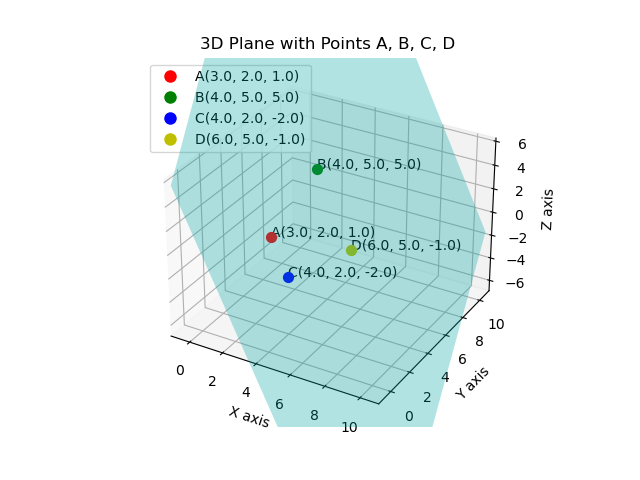
\includegraphics[width=\linewidth]{figs/fig.png}
   	\caption{Plot of the plane with points A, B, C and D}
\label{Plot}
\end{figure}
\end{document}
\end{document}
